\documentclass[en]{../../../../../../eplexam}

\hypertitle{Communication systems}{7}{ELEC}{2795}{2022}{Janvier}{All}
{Julien Giunta}
{Jérôme Louveaux, Claude Oestges and Charles Wiame (replacing Luc Vandendorpe)}

\section{Question 1}

Let us consider the downlink of a Wireless Local Area Network (WLAN), e.g. WiFi, operating
at 5 GHz in an indoor environment (at room temperature of 290 K). The system characteristics
are given as follows :

\begin{itemize}
    \item the channel bandwidth is 20 MHz,
    \item the modulation is QPSK,
    \item the EIRP at the access point (AP) is 32 mW,
    \itemthe antenna gain at the user equipement (UE) is 0 dB,
    \item the noise figure of the UE receiver (measured at 290 K) is 4.5 dB,
    \item the target SNR at the UE is 20 dB.
\end{itemize}

The path-loss $L$ expressed in [dB] is modeled as

$$L = 46 + 22 \log_{10} (d) + 10 n_w$$

where $d$ is the total distance in [m] and $n_w$ is the number of crossed walls.
When required, the wideband channel can be represented by three taps, characterized by the following power-delay profile.

\begin{table}[H]
    \centering
    \begin{tabular}{|c|c|c|}
        \hline
         Tap number & Relative power [dB] & Delay [ns]  \\
         \hline
         1 & 0 & 0 \\
         2 & -2 & 10 \\
         3 & -5 & 20 \\
         \hline
    \end{tabular}
    \caption{}
    \label{tab:my_label}
\end{table}

Finally, figure \ref{fig:auto-correlation} depicts the temporal auto-correlation of the narrowband channel when the UE
is moving on a straight line at 1 m/s.

\begin{figure}[H]
    \centering
    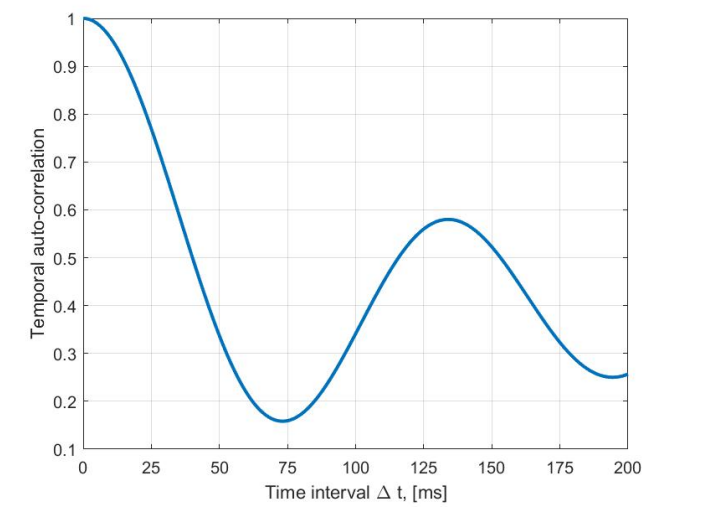
\includegraphics{Imgs/Channel_auto-correlation}
    \caption{Channel auto-correlation}
    \label{fig:auto-correlation}
\end{figure}


\paragraph{1.} We first consider that the radio channel is higly Ricean, so that we can neglect multipaths. What is the maximum possible range if we consider 0, 1 or 2 walls ? Detail the calculation.

\paragraph{2.} When considering multipaths, what is the delay-spread of the channel ? Should we consider that the transmission is frequency-flat or not ?

\paragraph{3.} To improve the performance, a spatial diversity technique is implemented at the UE, using two antennas. What could be a reasonable value for the antenna sepration to maximise the diversity gain ? Is it adequate for a smartphone ? a laptop ?

\nosolution
\newpage

\section{Question 2}

A digital transmission is performed on an AWGN channel with a memoryless linear modulation
at a symbol rate of 1 Mbaud (1Msymb/s), and using an SRRC (square root raised cosine) pulse
shaping filter $g(t)$ with roll-off factor $\alpah$ = 0.2. At the receiver, matched filtering is performed
and the signal is sampled at the symbol rate to provide the decision variable. Two possible
constellations are considered as represented below. The goal is to compare the performance of
the two constellations.

\begin{figure}[H]
    \centering
    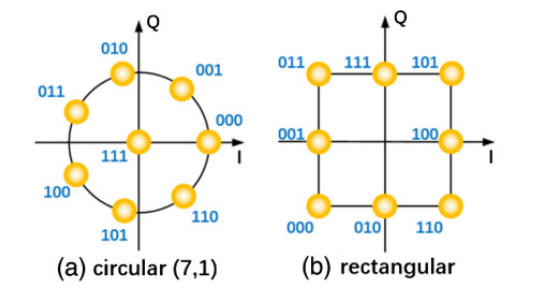
\includegraphics{Imgs/Constellations}
    \caption{Two constellations of size 8}
    \label{fig:my_label}
\end{figure}

\paragraph{1.} What is the decision rule for transmission on an ideal AWGN channel ? In particular,
(coarsely) draw the decision regions.

\paragraph{2.} For each of the constellations, assuming equiprobable symbols, determine its variance
as a function of the dimensions (you can choose yourself the parameter describing the
dimensions of each constellation).

\paragraph{3.} For each constellation, compute the SNR of the decision variable as a function of the
dimensions and of the noise variance.

\paragraph{4.} Compute an approximation of the \textbf{symbol} error probability for each of these constellations
in the presence of Gaussian noise, as a function of the SNR. Hint : you can use the nearest
neighbours approximation.

\paragraph{5.} Which one of the constellations performs better ?

\nosolution
\newpage

\section{Question 3}

One considers the relay system presented in the figure \ref{fig:relay_system}
\begin{figure}[H]
    \centering
    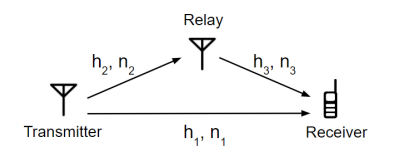
\includegraphics{Imgs/Relay_system}
    \caption{}
    \label{fig:relay_system}
\end{figure}

The following notations have been introduced :

\begin{itemize}
    \item $h_1$, $h_2$ and $h_3$ represent complex flat fading coefficients,
    \item $n_1(k)$, $n_2(k)$ and $n_3(k)$ represent independent noise sequences. These noise are all additive and white. In addition, they follow a complex Gaussian distribution : each real part and imaginary part follow the distribution $\mathcal{N}(0, \sigma^2)$.
\end{itemize}

The described system consists of :

\begin{itemize}
    \item \textbf{A transmitter}, sending a sequence $s(k)$ of independent and equiprobable symbols. These symbols come from a BPSK constellation and have unit energy. This sequence is sent to both the relay and the receiver simultaneously.

    \item \textbf{A relay}, receiving the signal given by $t(k) = h_2 \; s(k) + n_2(k)$. The relay directly forwards $t(k)$ to the receiver, without modifying it.

    \item \textbf{A receiver}, at which the following signals arrive :
    \begin{itemize}
        \item Direct signal from the transmitter : $r_1(k) = h_1 \; s(k) + n_1(k)$
        \item Signal forwarded via the relay : $r_2(k) = h_3 \; t(k) + n_3(k)$
    \end{itemize}
\end{itemize}

\paragraph{1.} It is first assumed that $h_2 = 1$ and that $h_1$ and $h_3$ are random, and model independent Rayleigh fading fluctuations. The values of these channels are perfectly estimated at the
receiver before data transmission. Give the diversity gain of the system. Briefly justify
your answer.\\


For the other questions, we now consider $h_1$, $h_2$ and $h_3$ deterministic, and known at the receiver.

\paragraph{2.} For this question, it is assumed that $r_2(k)$ arrives at the receiver with a delay of 1 compared to $r_1(k)$. The receiver therefore obtains a superposition given by

$$r_{tot} (k) = r_1(k) + r_2(k-1)$$

In order to compute an estimate of $s(k)$ based on $r_{tot}(k)$, one is interested in the Wiener
filter with two coefficients, such that

$$\hat{s}(k) = w(0) r_{tot}(k) + w(1) r_{tot}(k-1)$$

Provide the linear system to solve in order to obtain the filter coefficients w(0) and w(1).\footnote{As a reminder, some quantities are complex.} Detail your reasoning.

\paragraph{3.} In this question, the notion of delay is no longer present. It is now assumed that the
receiver is able to distinguish and to know $r_1(k)$ and $r2_(k)$ separately, for all time indexes.

\paragraph{(a)} Provide the ML problem to solve to estimate $s(k)$, based on both $r_1(k)$ and $r_2(k)$.\footnote{At the receiver, the ML detection is directly performed using signals $r_1(k)$ and $r_2(k)$. No other operation (e.g. filtering,...) is performed.}

\paragraph{(b)} By simplifying the ML problem, provide the decision variable to estimate $s(k)$.\footnote{ Hint : multiply $r_2(k)$ by a well-chosen term to obtain noise terms with equal variances in $r_1(k)$ and $r_2(k)$.}

\nosolution

\end{document}
